\documentclass[conference]{IEEEtran}
\IEEEoverridecommandlockouts
% The preceding line is only needed to identify funding in the first footnote. If that is unneeded, please comment it out.
\usepackage{cite}
\usepackage{amsmath,amssymb,amsfonts}
\usepackage{algorithmic}
\usepackage{graphicx}
\usepackage{textcomp}
\usepackage{xcolor}
\usepackage{listings}
\def\BibTeX{{\rm B\kern-.05em{\sc i\kern-.025em b}\kern-.08em
    T\kern-.1667em\lower.7ex\hbox{E}\kern-.125emX}}
\begin{document}

\title{RFID Sicherheit}


\author{\IEEEauthorblockN{Julian Hoever}
\IEEEauthorblockA{\textit{Verteilte Systeme} \\
\textit{Universität Duisburg-Essen}\\
Duisburg, Deutschland\\
julian.hoever@stud.uni-due.de}
}

\maketitle

\begin{abstract}
Die folgende Arbeit behandelt das Thema der RFID Sicherheit im Bezug auf Sicherheitslücken, Schutzmaßnahmen und Privatsphäre. Es werden einige mögliche Schwachstellen der RFID/NFC Technik aufgezeigt und Angriffstechniken vorgestellt, welche die zuvor aufgeführten Schwachstellen ausnutzen. Dabei wird darauf eingegangen, in welchen realen Szenarien diese Angriffe eine Bedrohung darstellen, wie zum Beispiel beim kontaktlosen Bezahlen oder der Diebstahlsicherung von Waren. Anschließend werden einige Schutzmaßnahmen skizziert, welche die zuvor genannten Angriffstechniken abmildern oder verhindern können und es wird diskutiert, wie durchführbar die genannten Angriffstechniken in der realen Welt sind. Dies hilft dabei abzuschätzen, wie relevant die Bedrohung ist, die von der RFID Technik in diesen Bereichen ausgeht. Abschließend wird noch der Aspekt der Einschränkung der Privatsphäre durch RFID Chips, besonders in Ausweisen aber auch in Produkten zur Diebstahlsicherung, besprochen und eingeordnet.
\end{abstract}

\section{Einleitung}
Die kontaktlose RFID Technik gehört bei vielen Menschen mittlerweile zum Alltag. Sie wird genutzt um kontaktlos Einkäufe zu bezahlen, auf der Arbeit mittels RFID Transponders die Eingangstür zu öffnen und bei einer Stempeluhr Arbeitszeiten zu dokumentieren. Die Einsatzbereiche der RFID Technik sind mittlerweile vielfältig. Eine weitere häufige Anwendung ist das Identifizieren von Gegenständen, zum Beispiel bei der Diebstahlsicherung von Waren oder der Verfolgung von Frachten. Durch die kontaktlosen Anwendungsbereiche bietet diese Technik einen erhöhten Komfort. Dafür wird häufig der Preis eines signifikant verringerten Sicherheitsniveaus oder eine Einschränkung der Privatsphäre gezahlt. Um eine Einschränkung der Sicherheit und Privatsphäre zu verhindern, müssen durch geeignete Schutzmaßnahmen Systeme die auf RFID beruhen abgesichert werden und dabei auch, falls erforderlich, Maßnahmen zu Schutz der Privatsphäre getroffen werden.

Aus diesem Grund wird in dieser Arbeit dargestellt, was die Probleme und möglichen Angriffsszenarien der RFID/NFC Technik sind. Dabei werden ausschließlich die passive RFID Transponder behandelt, da diese durch den einfachen Aufbau und das Fehlen einer eigenen Stromversorgung sehr weit verbreitet sind.

Zu Beginn wird dazu in Abschnitt 2 auf die Grundlagen der RFID/NFC Technik eingegangen. Anschließend beschreibt Abschnitt 3 was RFID/NFC konzeptionell für Schwachstellen besitzt. Darauf aufbauend wird dann in Abschnitt 4 erläutert was sich für mögliche Angriffe, auf die Sicherheit des Systems und die Privatsphäre der Nutzer, aus den in Abschnitt 3 genannten Schwachstellen ergeben. In Abschnitt 5 werden mögliche Sicherheitsmaßnahmen skizziert, welche Angriffe auf diese Technik erschweren und in Abschnitt 6 wird diskutiert wie durchführbar die vorgestellten Angriffe auf RFID Systeme in der Praxis überhaupt sind.

\section{Grundlagen}

\subsection{RFID Technik}
Radio Frequency Identification (RFID) ist eine Technik um kontaktlos Daten mittels eines Lesegerätes (Transceiver) aus einem Transponder auszulesen. Transponder gibt es in vielen verschiedenen Formen und Größen, je nach Anwendungsbereich. Grundlegend funktionieren alle Transponder aber recht ähnlich. Transponder bestehen in der Regel aus einer Antenne, in Form einer Spule, Schaltkreisen zum Senden/Empfangen und einem Speicher. Die Kommunikation erfolgt dann wie in Fig. \ref{fig1} dargestellt.

\begin{figure}[htbp]
\centerline{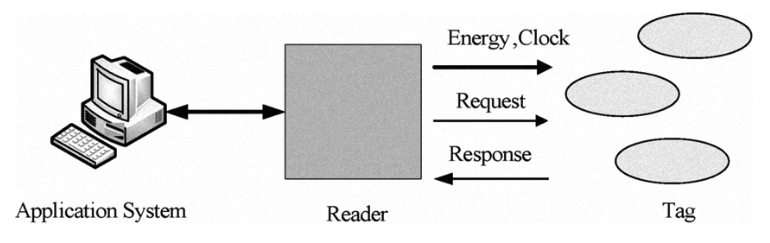
\includegraphics[width=0.5\textwidth]{img/kommunikation.png}}
\caption{Kommunikation zwischen Lesegerät (Reader) und Transponder \cite{b1}}
\label{fig1}
\end{figure}

Das Lesegerät (Reader) induziert über die spulenförmig angeordnete Antenne des Transponders, eine Spannung und Taktfrequenz, welche den Transponder mit dem nötigen Strom versorgt damit eine Kommunikation zwischen Lesegerät und Transponder stattfinden kann. Anschließend sendet das Lesegerät eine Anfrage an den Transponder, woraufhin ihm der Transponder seine Daten die er enthält übermittelt.

Das Frequenzspektrum von RFID ist hauptsächlich aufgeteilt in drei verschiedene Frequenzbänder. Diese Frequenzbänder sind:
\begin{itemize}
\item LF (Low frequency)
\item HF (High frequency)
\item UHF (Ultra high frequency)
\end{itemize}
Die Beschränkung von RFID auf diese drei Frequenzbänder ermöglicht es internationale Kompatibilität sicherzustellen \cite{b9}. Jedoch gibt es trotzdem in einigen Regionen leichte Abweichungen in den Frequenzen. Zum Beispiel nutzt Europa für das UHF Band die Frequenzen 866-868 MHz und die USA nutzt stattdessen die Frequenzen 902-928 MHz \cite{b9}. Fig. \ref{fig1.2} zeigt die Einordnung der Frequenzen in das Frequenzspektrum. Dabei werden für RFID hautsächlich die in Fig. \ref{fig1.2} markierten Frequenzen 125/134 kHz, 13.56 MHz, 868/915 MHz, 2.45 GHz, und 5.8 GHz genutzt. 

\begin{figure}[htbp]
\centerline{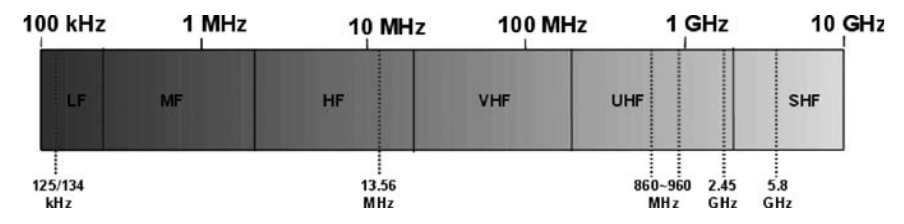
\includegraphics[width=0.5\textwidth]{img/frequenzen.png}}
\caption{Frequenzspektrum \cite{b9}}
\label{fig1.2}
\end{figure}

Abgesehen von den Frequenzbändern wird bei den RFID Transpondern unterschieden zwischen passiven und aktiven Transpondern.
\begin{itemize}
\item Passive Transponder besitzen keine eigene Spannungsquelle und erreichen dadurch lediglich eine Reichweite von weniger als 4 Metern \cite{b1}.
\item Aktive Transponder hingegen besitzen zusätzlich noch eine eingebaute Spannungsquelle, meist in Form einer Batterie. Dadurch sind Reichweiten von über 100 Metern möglich \cite{b1}.
\end{itemize}
Wie bereits in der Einleitung angemerkt fokussiert sich diese Arbeit ausschließlich auf die passiven Transponder, da diese in im alltäglichen Leben, im Gegensatz zu den aktiven Transpondern, von größerer Bedeutung sind.

\subsection{NFC Technik}
NFC steht für Near Field Communication und ist ein Standard der der mit einer Frequenz von 13.56 MHz und einer Übertragungsgeschwindigkeit von 424 KBit/s arbeitet \cite{b2}. Somit ist die NFC Technik auf dem High Frequency (HF) Frequenzband angesiedelt. Dieser Standard ist für Datenübertragungen von bis zu 10 cm ausgelegt und setzt technisch direkt auf der RFID Technik auf \cite{b2}. Dies ermöglicht mittels eines NFC Lesegeräts, beispielsweise Smartphones, sogar RFID Transponder auszulesen. Zum Lesen und Schreiben wird auch hier ebenfalls mit einer spulenförmigen Antenne gearbeitet.

NFC kann in 3 Betriebsmodi betrieben werden \cite{b2}:

\begin{itemize}
\item Peer-to-Peer Modus
\item Lese-Schreib Modus
\item Kartenemulationsmodus
\end{itemize}

Bei dem Peer-to-Peer Modus findet zwischen beiden Geräten ein bidirektionaler Datenaustausch statt. Ein Beispiel dafür ist der Datenaustausch zwischen zwei Smartphones per NFC. Dabei agieren beide Smartphones als Sender und Empfänger.

Bei dem Lese-Schreib Modus fungiert das aktive Gerät als Lesegerät und das passive Gerät ist hierbei ein kompatibler passiver RFID Transponder zum Beispiel in einem Aufkleber oder einer Karte mit eingebautem RFID Transponder. Es ist in diesem Modus aber auch möglich, dass das aktive Gerät einen RFID Transponder, welcher noch nie beschrieben wurde, beschreibt.

Bei dem Kartenemulationsmodus simuliert das NFC Gerät einen passiven RFID Transponder was bedeutet, das dieses Gerät keinerlei Berechnungen durchführt und lediglich die festgelegten Daten an ein anfragendes Lesegerät übermittelt. Dies findet zum Beispiel beim kontaktlosen Bezahlen mittels Smartphone Anwendung.

\section{Schwachstellen}
Die RFID und NFC Technik besitzt vielerlei Schwachstellen und diese sind zum Großteil sowohl auf RFID als auch auf NFC anzuwenden. Der wichtigste Unterschied zwischen RFID und NFC ist die Reichweite auf denen diese Technik operiert. Bei NFC muss der Angriff viel näher am Lesegerät stattfinden als bei RFID, da mit passiven RFID Transpondern Reichweiten von bis zu 4 Metern erreicht werden können. Im folgenden werden einige mögliche Schwachstellen beider Techniken aufgelistet.

\subsection{Authentifikation}
Wie bereits in dem Abschnitt mit den Grundlagen der RFID Technik beschrieben, übermittelt ein RFID Transponder im wesentlichen seinen gesamten Speicherinhalt an ein anfragendes Lesegerät. Das bedeutet, dass keinerlei Authentifikation auf Seiten des Transponders stattfindet und damit jedes Lesegerät was auf der Frequenz des Transponders agiert den Transponder lesen kann, wodurch möglicherweise Daten in falsche Hände gelangen können. Jedoch gibt es seit einiger Zeit Transponder, welche eine Authentifikation durchführen bevor Daten übermittelt werden.

\subsection{Lesegerät kennt Daten nicht}
Ein weiteres Problem ist, dass das Lesegerät, welches Daten von einem Transponder anfragt, nicht weiß was für Daten es von dem Transponder erhält. Diese Daten müssen aber trotzdem verarbeitet werden. Dies kann ohne Sicherheitsvorkehrungen dazu führen, dass verarbeitende Prozesse oder Datenbanken, welche diese Daten speichern sollen, Schaden nehmen können.

\subsection{Lesegerät muss Transponder lesen}
Ein RFID/NFC Lesegerät muss, wenn ein Transponder in seine Nähe kommt, diesen Transponder auch lesen. Ohne den Transponder zu lesen, kann das Lesegerät nicht entscheiden ob dieser Transponder wichtig ist oder nicht. Damit besteht von außen die Möglichkeit Reaktionen des Lesegerätes herbeizuführen \cite{b3}. Dies stellt ebenfalls ein Problem dar und lässt sich wie im nächsten Kapitel genauer erläutert ausnutzen.

\subsection{Eindeutige Identifikation}
Des Weiteren lässt sich sowohl der Speicherinhalt als auch die eindeutige Identifikationsnummer des Transponders dazu verwenden diesen zu identifizieren. Dies ist in vielen Situationen vermutlich gewünscht, kann aber auch ein Sicherheitsrisiko darstellen.

\subsection{Energieversorgung}
Damit ein passiver RFID Transponder funktionieren kann muss durch das Lesegerät eine Spannung induziert werden, welche dafür sorgt, dass der Transponder Daten versenden kann. Wird der RFID Transponder zum Beispiel durch einen Faradayschen Käfig abgeschirmt, wird der RFID Transponder nicht mit Energie versorgt und das Lesegerät bekommt keine Daten von dem RFID Transponder übermittelt.

\subsection{Übertragung}
Ursprünglich ist RFID mit dem Standard ISO/IEC 18000 so standardisiert worden, dass die Übertragung zwischen Lesegerät und Transponder im Klartext geschieht. Dies sorgt dafür, dass die Übertragung abgehört werden kann.

\section{Angriffe auf Sicherheit und Privatsphäre}
Mit den im vorherigem Abschnitt beschriebenen Schwachstellen lassen sich mögliche Angriffsszenarien beschreiben welche die Sicherheit eines Systems ohne entsprechende Gegenmaßnahmen gefährden würden.

\subsection{Kopieren von Transpondern}
Bei der Verwendung von Transpondern ohne Authentifikation lässt sich der Transponder ohne weiteres mit einem kompatiblen Lesegerät auslesen. Die ausgelesenen Daten können anschließend dazu verwendet werden einen neuen uninitialisierten Transponder zu beschreiben um dadurch eine Kopie des ursprünglich gelesenen Transponders zu erhalten. Diese Kopie kann dann den gleichen Zweck erfüllen wie das Original. Angenommen der Originaltransponder wurde dazu verwendet eine Haustüre zu öffnen. Das bedeutet, dass es durch ein kurzes Auslesen des Originaltransponders möglich ist einen zweiten Hausschlüssel zu erzeugen. 

Diese Kopiervorgänge können innerhalb weniger Sekunden geschehen und brauchen nur einen flüchtigen Kontakt mit dem Originaltransponder. Dies kann zum Problem werden, wenn beispielsweise ein RFID Transponder an einem Schlüsselbund oder eine Karte in einer Brieftasche kurz aus den Augen gelassen wird. In der Zeit könnte ein Angreifer, ohne Aufmerksamkeit zu erregen, die Daten der jeweiligen Transponder kopiert haben.

\subsection{Kom­pro­mit­tie­ren des Lesegerätes}
Die Möglichkeit einfach einen RFID/NFC Transponder auszulesen stellt nicht nur ein Problem für die Sicherheit der Daten auf dem Transponder da. Durch das einfache Auslesen kann auch die Sicherheit des Lesegerätes und der darunter liegenden Softwareinfrastruktur entstehen. Dieses Problem entsteht dadurch, dass ein Lesegerät jeden Transponder liest, welcher sich in Reichweite ist. Befindet sich unter diesen Transpondern ein Transponder welcher Schadcode als Daten enthält, wird das Lesegerät, beispielsweise ein Smartphone oder eine Türsteuerung, dessen Daten ebenfalls lesen und verarbeiten. Wird auf Seiten des Lesegerätes nun nicht dafür gesorgt, dass Schadcode unschädlich gemacht wird, kommt dieser Schadcode ungehindert in tiefere Systembereiche.
Durch die verhältnismäßig kleine Speichergröße eines RFID Transponders von Bytes bis wenigen Kilobytes, beispielsweise 4 kB bei der MIFARE Classic EV1 4K \cite{b4}, ist die Größe des Schadcodes begrenzt, reicht aber aus um Schaden anzurichten \cite{b5}. Bei dem Schadcode kann es sich beispielsweise um SQL Injections handeln. Ein Beispielszenario wäre, dass ein Transponder mit einem schädlichen SQL Statement wie
\begin{lstlisting}[xleftmargin=.07\textwidth, xrightmargin=.07\textwidth]
"; DROP TABLE <tabellenname>
\end{lstlisting}
\cite{b5} präpariert worden ist und dieser dann in die Nähe eines Lesegerätes gebracht wird. Das Lesegerät würde dann die Daten lesen und möglicherweise versuchen diese Daten in eine Datenbank zu schreiben. Das würde in der Datenbank dafür sorgen, dass die Tabelle mit dem in der SQL Injection angegebenen Tabellennamen gelöscht wird. Durch den Datenverlust entstehen in der Regel schwere Schäden auf Seiten des Lesegerätes und der dahinterstehen Softwareinfrastruktur.

\subsection{Erweitern von NFC zu Bluetooth}
Ein ähnliches Problem, was aber speziell NFC betrifft, ist die Koppelung von Bluetooth Verbindungen mittels NFC oder das Teilen von größeren Datenmengen eingeleitet über NFC. Dieses Angriffsszenario betrifft hauptsächlich Smartphones. Smartphones mit NFC besitzen oft die Möglichkeit über NFC Bluetooth Verbindungen herzustellen oder Daten zu teilen indem lediglich das Smartphone in die Nähe des anderen Gerätes gebracht wird. Beim Teilen von größeren Datenmengen über NFC wird auch häufig NFC nur zum Koppeln einer Bluetooth Verbindung genutzt und der eigentliche Datentransfer läuft anschließend über diese Bluetooth Verbindung \cite{b6}. Das Problem dabei ist, dass so die Kurzstreckenverbindung über NFC erweitert wurde auf eine Bluetooth Verbindung mit einer deutlich erhöhten Reichweite und einer schnelleren Übertragungsrate \cite{b6}. Diese Verbindung kann anschließend dafür genutzt werden aus größerer Entfernung Schadcode auf das Zielgerät zu schleusen.

\subsection{Tracking durch Transponder IDs}
Ein weiteres Problem ist die eindeutige Identifikationsnummer eines RFID Gerätes. Jedes RFID Gerät besitzt eine eindeutige Identifikationsnummer welche benötigt wird um Kollisionen bei der Übertragung zu verhindern \cite{b3}. Diese Identifikationsnummer bestimmt jeden Transponder und jedes RFID Gerät (und damit auch NFC Gerät) eindeutig und ermöglicht ein Tracking dieser Geräte. Dadurch kann massiv die Privatsphäre von Personen beeinträchtigt werden. Ein Szenario in dem diese Technik ausgenutzt werden könnte ist beispielsweise ein Unternehmen, in dem jeder Mitarbeiter RFID Transponder zum Zeitstempeln an Stempeluhren, Bezahlen in der Mensa und/oder zur Zugangskontrolle besitzt. Das Unternehmen könnte in dem Betrieb an vielen verschiedenen Stellen RFID Lesegeräte installieren. Diese Lesegeräte würden die Identifikationsnummer jedes RFID Transponders lesen, welcher in seine Reichweite kommt. Die Identifikationsnummer lassen sich dann Mitarbeitern zuordnen. Dadurch ist es möglich unbemerkt sämtliche Bewegungen der Mitarbeiter im Gebäude zu verfolgen. Diese Bewegungsprofile könnten anschließend dazu genutzt werden deren Arbeitszeit zu überwachen oder personelle Entscheidungen zu treffen.

Diese Art des Trackings wäre beispielsweise auch beim Einkaufen ein Problem. Geschäfte könnten an diversen Stellen im Laden RFID Lesegeräte platzieren und die Produkte mit RFID Transpondern zur Diebstahlsicherung ausstatten. Nimmt nun ein Kunde ein Produkt, und bewegt sich anschließend durch das Geschäft, registriert jedes Lesegerät, an dem der Kunde vorbei geht, die eindeutige Kennung des RFID Transponders. Dadurch wären die Geschäfte in der Lage das Konsumverhalten und die Laufwege der Kunden zu überwachen und so kann der gesamte Einkaufsprozess dieser Person genaustens nachverfolgt werden. Dies stellt ebenfalls eine erhebliche Gefährdung der Privatsphäre des Kunden dar.

\subsection{Denial of Service Angriffe}
Ebenfalls im Einzelhandel ist nicht nur das Tracking mittels RFID Transpondern ein Problem. Ein anderer wichtiger Angriff gegen RFID/NFC Technologie ist der Denial of Service. Beim Denial of Service Angriff geht es darum die Funktionsfähigkeit von RFID Transpondern oder Lesegeräten zu behindern, oder auch ganz funktionsunfähig zu machen. Diesen Punkt kann man aus zwei Perspektiven beleuchten. Entweder kann es darum gehen den Transponder funktionsunfähig zu machen oder es kann darum gehen ein Lesegerät funktionsunfähig zu machen. Beide Punkte werden im folgenden erläutert:

\subsubsection{Angriff auf Transponder}
Bei einem Denial of Service Angriff auf einen Transponder handelt es sich überwiegend um einen Angriff auf die Stromversorgung des Transponders. Mit einem solchen Angriff soll die Stromversorgung mittels Induktion verhindert werden. Dadurch kann der Transponder erst gar nicht aktiv werden und auch keine Daten austauschen. Eine Möglichkeit dies zu erreichen, ist es den Transponder durch einen so genannten Faradayschen Käfig abzuschirmen wie in Fig. \ref{fig2} dargestellt.

\begin{figure}[htbp]
\centerline{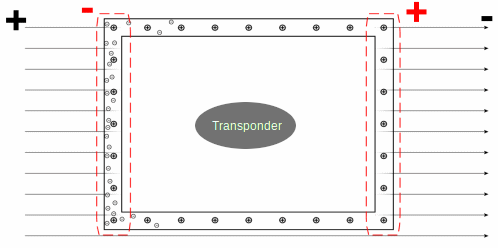
\includegraphics[width=0.5\textwidth]{img/kaefig.png}}
\caption{Transponder im Faradayschen Käfig \cite{b7}}
\label{fig2}
\end{figure}

Bei einem Faradayschen Käfig handelt es sich um eine vollständig geschlossene leitende Hülle. Wirkt ein elektrisches Feld auf diese Hülle ein sorgt der Faradaysche Käfig dafür, wie in Fig. \ref{fig2} dargestellt, dass dieses elektrische Feld nicht in das innere der Hülle vordringen kann. Das elektrische Feld ist in der Grafik dargestellt durch die waagerechten Linien und die Hülle als der rechteckige Kasten.

Für einen Transponder der in einen solchen Faradayschen Käfig gebracht wird, bedeutet dies, dass das vom Lesegerät erzeugte elektrische Feld zur Stromversorgung durch den Faradayschen Käfig abgehalten wird und nicht in das innere dieses Käfigs vordringen kann. Damit wird der, im inneren befindliche, Transponder nicht mit der nötigen Energie versorgt und es findet kein Datenaustausch zwischen Lesegerät und Transponder statt. Für das Lesegerät wirkt es so als sei der Transponder überhaupt nicht existent.

Ein daraus resultierendes Angriffsszenario wäre beispielsweise die Diebstahlsicherung von Waren im Einzelhandel. Bei der Diebstahlsicherung von beispielsweise Kleidung werden RFID Transponder dazu genutzt um einen Alarm auszulösen, wenn eine Person, ohne die Kleidung zu bezahlen, den Laden verlässt. Dieses unbefugte Verlassen des Ladens wird von RFID Lesegeräten am Ausgang des Ladens bemerkt, indem die RFID Transponder in den Kleidungsstücken beim Durchqueren der Lesegeräten erkannt werden. Wurde das Diebesgut aber vor Verlassen des Ladens in einen Faradayschen Käfig verstaut kann die Person den Laden verlassen ohne das die Lesegeräte am Ausgang Alarm schlagen. Dies kann unter Umständen für einen Einzelhändler hohe Verluste bedeuten.

\subsubsection{Angriff auf Lesegeräte}
Eine andere Möglichkeit einen Denial of Service Angriff durchzuführen ist, indem man versucht ein Lesegerät funktionsunfähig zu machen. Dabei wird ausgenutzt, dass ein aktives RFID/NFC Lesegerät jeden RFID/NFC Transponder in seiner Umgebung auslesen muss um zu entscheiden ob er wichtig für die Anwendung des Lesegerätes ist. Dieser Lesevorgang eines Transponders dauert einen kleine Zeitspanne, in der das Lesegerät nicht in der Lage ist andere Transponder zu lesen. Das bedeutet es gibt die Möglichkeit ein Lesegerät für einen kurzen Moment zu blockieren \cite{b3}.

Mit der Möglichkeit, das Lesegerät für einen kurzen Moment zu blockieren, lassen sich so genannte Jammer bauen. Ein Jammer ist ein Gegenstand auf dem eine große Anzahl an RFID Transpondern installiert ist. Gelangt so ein Jamming Gerät in die Reichweite eines Lesegerätes, kann dieses Lesegerät, durch die hohe Anzahl an gleichzeitigen Antworten, funktionsunfähig gemacht werden. Dies kann ebenfalls dafür genutzt werden um beispielsweise eine Diebstahlsicherung von Waren zu umgehen. Wenn man mit einer Ware mit RFID Transponder und dem Jammer durch die Lesegeräte am Ausgang des Geschäftes geht, sind diese Lesegeräte mit der Anzahl der RFID Transpondern überfordert und schlagen ebenfalls keinen Alarm.

\subsection{Abhören der Kommunikation}
Anstatt die Übertragung mittels Denial of Service Angriffe zu unterbinden, kann es auch von Interesse sein eine Übertragung abzuhören. Dies ist möglich, da die Kommunikation, nach ISO/IEC 18000, zwischen Lesegerät und Transponder grundlegend ohne Verschlüsselung stattfindet \cite{b3}. Der Grund für die meist fehlende Verschlüsselung bei der Kommunikation sind die Kosten und der Aufwand der damit verbunden ist. Jedoch ist die Technik dadurch verwundbar, was in einigen Situationen ein Problem darstellt.

Ein Angriff sieht wie folgt aus. Ein Angreifer begibt sich mit einem passenden Lesegerät in die Reichweite eines anderen Lesegerätes bei dem gerade eine Kommunikation zwischen Lesegerät und Transponder stattfindet. Der Angreifer kann über sein Lesegerät die Daten, die zwischen den legitimen Lesegerät und Transponder ausgetauscht werden, abhören und aufzeichnen. Wenn der Angreifer die Daten aufgezeichnet haben sollte, kann er diese Daten zu einem späteren Zeitpunkt dazu nutzen um diese selber an das Lesegerät zu versenden und damit eine Kommunikation mit dem echten Transponder vorzutäuschen \cite{b8}. 

Ein anderes Problem ist dass die gesammelten Informationen auch sensible personenbezogene Daten enthalten können, was eine Einschränkung der Privatsphäre bedeutet, wenn man diese Daten unverschlüsselt im Klartext überträgt.

\subsection{Man-In-The-Middle Angriff}
Eine Angriffstechnik die auf den zuvor beschriebenen Angriff aufbaut, ist der so genannte Man-In-The-Middle (MITM) Angriff. Bei dieser Angriffstechnik handelt es sich grundsätzlich um eine Kombination aus mehreren Angriffstechniken. Ein Man-In-The-Middle Angriff ist eine Kombination aus Abhören von Daten, Verändern von Daten und Weitersenden von Daten. Dabei beruht dieser Angriff stark auf der Schwachstelle, dass die Kommunikation zwischen RFID Lesegerät und Transponder unverschlüsselt stattfindet. In Fig. \ref{fig3} ist der Ablauf eines solchen Angriffs schematisch dargestellt.

\begin{figure}[htbp]
\centerline{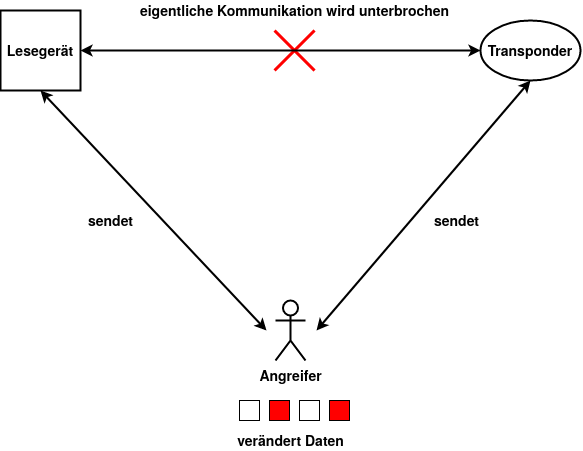
\includegraphics[width=0.5\textwidth]{img/MITM.png}}
\caption{Ablauf eines Man-In-The-Middle Angriffs}
\label{fig3}
\end{figure}

Für einen Man-In-The-Middle Angriff muss der Angreifer in der Lage sein die eigentliche Kommunikation zwischen Lesegerät und Transponder zu unterbrechen. Ist die Unterbrechung erfolgt muss nahtlos die die Kommunikation über den Angreifer umgeleitet werden, damit das Lesegerät diese Unterbrechung nicht bemerkt. Ist dieses Umleiten über den Angreifer erfolgreich durchgeführt worden, werden sämtliche Nachrichten die zwischen Lesegerät und Transponder ausgetauscht werden zuerst über den Angreifer weitergeleitet, der diese dann ebenfalls an den Transponder oder das Lesegerät weiterleitet. Dadurch ist der Angreifer in der Lage die gesamte Kommunikation zwischen Lesegerät und Transponder aufzuzeichnen ohne dass das Lesegerät diese Umleitung bemerkt.

Das Umleiten der Kommunikation ist in Fig. \ref{fig3} dargestellt als Doppelpfeil von Lesegerät zu Angreifer und Angreifer zu Transponder. Das rote Kreuz stellt die unterbrochene Kommunikation zwischen Lesegerät und Transponder dar.

Der Angreifer ist jedoch nicht nur in der Lage die Kommunikation zu belauschen. Da er sich unbemerkt zwischen der Kommunikation von Lesegerät und Transponder befindet und im Prinzip nur die Nachrichten weiterleitet die er erhält, ist er auch in der Lage die Nachrichten vor der Weiterleitung zu modifizieren oder blockieren. Der Transponder oder das Lesegerät ist dabei nicht in der Lage zu entscheiden ob die Pakete tatsächlich von dem legitimen Kommunikationspater oder von einem Angreifer kommen. Dadurch ist der Angreifer in der Lage falsche Informationen zu verteilen und den Datenaustausch zwischen Lesegerät und Transponder zu steuern wie es ihm beliebt.

Dies stellt ein erhebliches Problem im Bezug auf das Vertrauen und die Datenintegrität einer RFID/NFC Kommunikation dar.

\section{Sicherheitsmaßnahmen}
Nun wurden eine Reihe von Schwachstellen und Angriffstechniken beleuchtet, welche ernsthafte Probleme für die Sicherheit und Privatsphäre der Nutzer solcher Systeme darstellen. Viele der Schwachstellen wurden im Laufe der Jahre bereits behoben oder sind nur noch teilweise vorhanden. Aus diesem Grund werden als nächstes Sicherheitsmaßnahmen vorgestellt, die die schwere der vorgestellten Schwachstellen abmildern können, oder sogar ganz verhindern können. Dazu wird für jede Schwachstelle separat beleuchtet, wie dieses Problem abgesichert werden kann. Generell gilt für viele der hier vorgestellten Sicherheitsmaßnahmen, dass je leistungsfähiger ein Transponder ist, desto mehr Sicherheit ist potenziell möglich. Dies spiegelt sich dann aber auch im Preis des Transponders wieder. Damit muss für jede Anwendung abgewogen werden wie viel Sicherheit für ein System benötigt wird.

\subsection{Authentifikation}
Wie bereits in dem vorherigen Abschnitt gesehen, stellt es ein großes Problem dar, wenn ein Transponder ohne Authentifizierung ausgelesen werden kann. Besonders wenn dieser Transponder für sicherheitskritische Systeme wie Türsteuerungen eingesetzt wird. Dies würde das einfache Auslesen und Kopieren eines Transponders ermöglichen. Um dieses Problem zu verhindern ist es notwendig eine Authentifizierung vor Datenaustausch mit dem Transponder durchzuführen. Dazu gibt es verschiedene Ansätze, die eine Authentifizierung zwischen Lesegerät und Transponder realisieren. Die Ansätze unterscheiden sich im wesentlichen an deren Sicherheit und Komplexität. Im folgenden wird der Ansatz der MIFARE Classic EV erläutert \cite{b4}, jedoch gibt es noch diverse  weitere Möglichkeiten.

Der MIFARE Classic EV1 ist ein RFID Transponder, der auf dem NFC Frequenzband (HF) mit einer Frequenz von 13.56 MHz und einer Reichweite von 10 cm agiert \cite{b4}. Dieser leistungsfähige Transponder ist in der Lage Berechnungen durchzuführen was bei der Authentifizierung genutzt wird. Der Speicher dieses Transponders ist aufgeteilt in Sektoren und jeder Sektor ist nochmals unterteilt in 16 Byte Blöcke. Jeder Sektor kann von dem Lesegerät separat ausgelesen werden und für jeden Sektor muss eine separate Authentifizierung zwischen Lesegerät und Transponder erfolgen. Um für jeden Sektor eine eigenständige Authentifikation durchzuführen, ist der letzte Block eines jeden Sektors (Sector Trailer) wichtig. Dieser Block enthält drei Informationen: Einen Schlüssel A, Zugriffsbedingungen und optional noch einen Schlüssel B. Für die eigentliche Authentifikation nutzt der MIFARE Classic EV1 ein so genanntes Drei-Phasen-Authentifizierungsprotokoll. Der Ablauf dieses Protokolls ist in Fig. \ref{fig4} schematisch dargestellt.

\begin{figure}[htbp]
\centerline{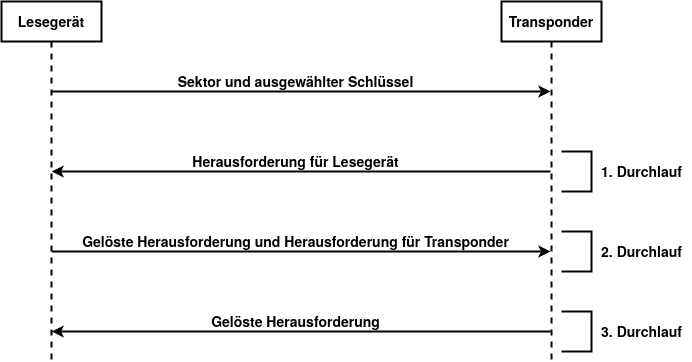
\includegraphics[width=0.5\textwidth]{img/three_pass.png}}
\caption{Drei-Phasen-Authentifikation der MIFARE Classic}
\label{fig4}
\end{figure}

Zu Beginn der Authentifizierung wählt das Lesegerät den Sektor aus, der gelesen werden soll und wählt einen Schlüssel A oder B des Transponders aus, der für die Authentifizierung verwendet werden soll. Diese Daten sendet das Lesegerät an den Transponder. 

Anschließend, im ersten Durchlauf der Drei-Phasen-Authentifizierung, ließt der Transponder aus dem Sector Trailer für den angefragten Sektor den gewünschten Schlüssel und die Zugriffsbedingungen aus. Zum Abschluss des ersten Durchlaufs antwortet der Transponder dem Lesegerät, indem er dem Lesegerät eine Zahl als Herausforderung (Challenge) sendet. Ab dem Punkt wo das Lesegerät diese Zahl erhält, ist die weitere Kommunikation zwischen Lesegerät und Transponder verschlüsselt.

Nachdem das Lesegerät die Zahl vom Transponder erhalten hat, beginnt der zweite Durchlauf. Das Lesegerät berechnet mittels des gewählten Schlüssels und zusätzlichen Informationen eine Antwort auf die Herausforderung. Daraufhin sendet das Lesegerät die Antwort auf die Herausforderung und zusätzlich eine Zahl als Herausforderung für den Transponder an den RFID Transponder. Damit ist der zweite Durchlauf beendet.

Im dritten und letzten Durchlauf erhält der Transponder die gelöste Herausforderung vom Lesegerät und verifiziert die Korrektheit der Lösung. Ist dies der Fall, berechnet der Transponder die Lösung zu der Herausforderung  vom Lesegerät und sendet diese Lösung wieder zurück zum Lesegerät. Das Lesegerät verifiziert diese Lösung ebenfalls und wenn die Lösung korrekt ist, ist die Authentifizierung damit erfolgreich abgeschlossen.

Das bedeutet diese Art der Authentifikation beruht darauf, dass beide Kommunikationspartner den korrekten Schlüssel für den jeweiligen Sektor besitzen. Dies hat den Vorteil, da das Lesegerät nur Sektoren des Transponders lesen kann für den es auch den geheimen Schlüssel kennt. Damit ist ein effektives Berechtigungsmanagement möglich, indem jedem Lesegerät nur die Schlüssel für Sektoren bereitgestellt werden, die es auch lesen können soll.

Die beschriebene Art der Authentifizierung stellt damit eine Möglichkeit dar RFID Transponder vor unberechtigtem Kopieren und vervielfältigen zu schützen. Jedoch wird für diese Methode ein Transponder vorausgesetzt, welcher über eine größere Leistung verfügt um Berechnungen durchführen zu können und zufällige Herausforderungen generieren zu können. Eine andere einfachere Methode wäre wenn das Lesegerät dem Transponder ein einfaches Passwort übermitteln würde und der Transponder dieses Passwort dann lediglich nur mit dem korrekten Passwort abgleicht. Diese Methode hat aber die große Schwachstelle, dass die Übertragung des Passwortes im Klartext erfolgt und somit mitgelesen werden kann. Dadurch wäre die Sicherheit des Passwortes gefährdet, was dazu führt, dass die Transponder wieder kopiert werden können. Aus diesem Grund ist die Methode wie vom MIFARE Classic EV1 implementiert, der einfachen Passwort Methode zu bevorzugen.

Eine weitere Möglichkeit, die zusätzlich neben einer einer starken Authentifizierung für Sicherheit sorgt, ist das Verringern des Funktionsradius eines RFID Transponders. Damit wird es erschwert aus der Distanz Kopierversuche zu unternehmen. Beispielsweise wird das beim kontaktlosen Bezahlen mittels Bankkarten so gemacht.

\subsection{Lesegerät kennt Daten nicht}
Ein weiteres Problem von RFID Systemen ist es dass das Lesegerät die Daten des Transponder auslesen und verarbeiten muss. Jedoch kann es, wie im vorherigen Abschnitt gesehen, sein, dass die Daten des Transponders Schadcode wie SQL Injections enthalten. Wenn diese so wie sie sind, beispielsweise von einer Datenbank, verarbeitet werden, kann dadurch ein beachtlicher Schaden entstehen. Aus diesem Grund müssen die Daten vor der Weitergabe in tiefere Softwarestrukturen vorverarbeitet werden oder erst gar nicht Daten von unautorisierten Transpondern zu lesen.

Sich nur darauf zu verlassen, dass ein Transponder, der sich erfolgreich bei einem Lesegerät autorisieren konnte, nur ungefährliche Daten übermittelt ist gefährlich. Es kann durchaus sein, dass es eine unentdeckte Schwachstelle bei der Autorisierung vorliegt und diese genutzt wurde um einen Transponder mit Schadcode zu generieren, der sich problemlos autorisieren kann. Wenn sich nur auf eine einwandfreie Autorisierung verlassen wird, würde in dem Fall der Schadcode trotzdem ungehindert in das Softwaresystem vordringen können.

Jedoch kann man zusätzlich die Daten, die man von einem autorisierten RFID Transponder liest, vorverarbeiten um zusätzlich das Eindringen von Schadcode in tiefere Softwarestrukturen zu verhindern. Eine Möglichkeit ist, die Eingabedaten zu in Form eines Strings, vor der Weitergabe in tiefere Systembereiche mit Escape-Sequenzen zu versehen. Dies sorgt dafür, dass bei der Verarbeitung oder Speicherung dieser Daten von einer Datenbank kein Schadenspotential mehr besteht.

Generell sollten beim Entwurf von RFID Systemen darauf geachtet werden, dass die Daten, die von einem RFID Transponder übermittelt werden, immer mit großer Vorsicht verarbeitet werden. Diese Daten müssen wie Nutzereingaben gesehen werden und es darf sich nicht auf die Richtigkeit dieser Daten verlassen werden.

Ein Problem bei dem es auch darum ging, dass Daten mit Schadcode auf ein Lesegerät übertragen werden war das Erweitern von NFC auf Bluetooth. Viele IoT Geräte und Smartphones besitzen die Möglichkeit mittels NFC eine Bluetooth-Verbindung zu etablieren. Über diese Bluetooth-Verbindung kann dann Schadcode auf das Zielgerät geladen werden. Um dies zu verhindern besteht erneut die Möglichkeit dass sich die beiden Geräte vor der Koppelung mit Bluetooth über NFC authentifizieren müssen. Weiter sollte bei jedem Koppelungsversuch, sei es auch nur zum Übertragen kleinerer Datenmengen, der Nutzer nach seinem ausdrücklichen Einverständnis gefragt werden. Damit kann die Sicherheit dieser technischen Möglichkeit verbessert werden.

\subsection{Lesegerät muss Transponder lesen}
Die Schwachstelle, dass das Lesegerät den RFID Transponder lesen muss wenn er in Reichweite kommt, hatte, wie in einem vorherigen Abschnitt dargestellt wurde, zur Folge, dass es möglich war eine Lesegerät mittels Denial of Service Angriff zu blockieren. Dies war über die so genannten Jamming Geräte möglich. Diesem Problem kann man entgegenwirken, indem man ein Antikollisionsverfahren implementiert. Jedoch kann dadurch ein Angriff durch Denial of Service nur erschwert werden aber nicht verhindert werden.

\subsection{Energieversorgung}
Eine andere Art des Denial of Service ist es, wie in einem vorherigen Abschnitt gesehen, wenn man einen Transponder mittels Faradayschen Käfig abschirmt. Dadurch wird die Energieversorgung des Transponders unterbunden und es können keine Daten gelesen werden, beziehungsweise für das Lesegerät ist dieser Transponder gar nicht sichtbar. Diese Schwachstelle von RFID Systemen stellt, wie bereits erläutert, in der Diebstahlsicherung ein großes Problem dar, da es möglich ist unbemerkt Ware durch die Lesegeräte am Ausgang eines Geschäftes zu schmuggeln.

Es ist aber nicht ohne weiteres möglich diese Schwachstelle abzusichern, da RFID darauf beruht die Transponder über ein elektrisches Feld mit Energie zu versorgen. Aus diesem Grund stellt die Abschirmung der Transponder mittels eines Faradayschen Käfigs ein ernsthaftes Problem für diese Technik dar. Um die Schwere dieses Problems abzumildern, kann sie mit anderen Techniken kombiniert werden, wie zum Beispiel Videoüberwachungssysteme oder den Einsatz eines Ladendetektiv. Es muss sich individuell für jedes RFID System überlegt werden wie mit dem Problem der Abschirmung umgegangen werden soll.

\subsection{Eindeutige Identifikation}
Jeder RFID Transponder besitzt eine eindeutige Kennung mit der es möglich ist ein Tracking von RFID Transpondern durchzuführen. Dazu wurden in einem vorherigen Abschnitt das Szenario von der Verfolgung von Mitarbeitern in einem Unternehmen durch RFID Transponder und die Verfolgung von Kunden in einem Geschäft diskutiert. Dies waren beides Szenarien die massiv die Privatsphäre von Menschen beeinträchtigt haben. Um diesem Problem entgegenzuwirken gibt es auch hier wieder verschiedene Ansätze.

Um Tracking vollständig zu unterbinden kann ein Transponder jedes Mal wenn er von einem Lesegerät gelesen wird eine zufällige ID generieren und dem Lesegerät zusenden. Dadurch kann ein Lesegerät zu einem späteren Zeitpunkt einen bereits gelesenen Transponder nicht wiedererkennen, da sich die ID des Transponders in beiden Lesevorgängen unterscheidet. Jedoch hat diese Art der vollständigen Anonymisierung auch Nachteile. Möglicherweise ist es in manchen Anwendungen gewünscht, dass Transponder bestimmten Personen oder dem System selber zugeordnet werden können.

Eine Möglichkeit dieses Problem zu lösen ist das randomisierte HashLock Schema von Weis, Sarma, Rivest und Engels \cite{b9}. Bei diesem Ansatz wird bei jedem Auslesen eines Transponders eine andere Identifikationsnummer übermittelt. Der Ablauf der randomisierten HashLock Variante wird in Fig. \ref{fig5} dargestellt.

\begin{figure}[htbp]
\centerline{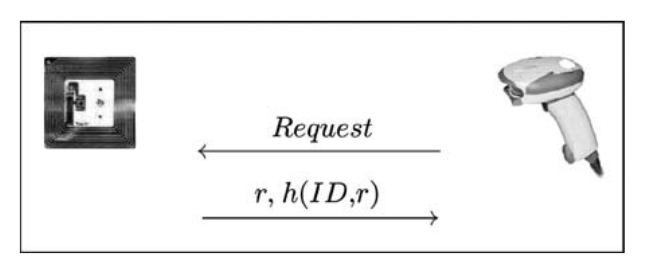
\includegraphics[width=0.5\textwidth]{img/hashlock.png}}
\caption{Ablauf des randomisierten HashLock Schemas \cite{b9}}
\label{fig5}
\end{figure}

Jeder Transponder besitzt bei diesem Verfahren eine eindeutige Identifikationsnummer ($ID$), die sich systemintern zuordnen lässt. Liest nun ein Lesegerät diesen RFID Transponder aus, generiert dieser Transponder eine Nonce $r$. Diese Nonce ist eine zufällige Zahl welche nach Möglichkeit nur ein Mal verwendet werden darf. Anschließend berechnet der Transponder aus der Nonce $r$, der geheimen Identifikationsnummer $ID$ und einer Hashfunktion $h$ einen Hash $h(ID, r)$. 

Eine Hashfunktion ist eine nicht umkehrbare Funktion, welche eine Eingabe auf eine (in der Regel) kleiner Ausgabe abbildet. Eine Hashfunktion sollte dabei möglichst für jede Eingabe auf eine andere Ausgabe abbilden, was bei einer kleineren Ausgabemenge nicht möglich ist.

Wurde der Hash $h(ID, r)$ vom Transponder berechnet, sendet dieser, wie in Fig. \ref{fig5} dargestellt, das Ergebnis des Hashes und zusätzlich die Nonce $r$ zurück an das Lesegerät. Die Anwendung die die Daten des Lesegerätes verarbeitet kann dann, die in einer Datenbank gespeicherten Identifikationsnummern aller systemzugehörigen Transponder vergleichen ob eine Identifikationsnummer gehasht mit der Nonce den gleichen Hash ergibt wie der übermittelte Hash.

Dieses Vergleichen aller Identifikationsnummern mit dem übermittelten Hash ist eine sehr rechenaufwendige Operation \cite{b9}. Es gibt aber noch weitere Ansätze die sich diesem Problem annehmen. Des Weiteren sollte dieses randomisierte HashLock Verfahren nicht, ohne zusätzliche Authentifikation, zum authentifizieren von Transpondern genutzt werden, da es einen effektiven und simplen Angriff gegen dieses Verfahren gibt \cite{b9}.

Ein Angreifer könnte den Austausch der gehashten Identifikationsnummer und der Nonce mitschneiden. Dies ist möglich, da die Kommunikation zwischen Lesegerät und Transponder unverschlüsselt erfolgt. Anschließend kann der Angreifer diesen mitgeschnittenen Hash und Nonce dazu nutzen sich selber bei dem Lesegerät zu authentifizieren. Aus diesem Grund sollte dieses Verfahren nur in Kombination mit anderen Authentifikationsverfahren verwendet werden.

\subsection{Übertragung}
Ein weiteres beschriebenes Problem ist dass die Übertragung zwischen Lesegerät und Transponder im Klartext stattfindet. Dies sorgt dafür, dass die Kommunikation von einem Angreifer mitgeschnitten werden kann. Daraus resultiert eine ganze Reihe an Schwachstellen. Zum einen ermöglicht das Fehlen einer Verschlüsselung in RFID Kommunikation die oben beschriebenen Man-In-The-Middle Angriffe. Zum anderen bedeutet die fehlende Verschlüsselung aber auch Probleme für Protokolle wie das im Unterkapitel "Eindeutige Identifikation" des Abschnitts "Sicherheitsmaßnahmen" beschriebene HashLock Verfahren \cite{b9}. Aus diesem Grund muss eine Kommunikation zwischen RFID Lesegerät und Transponder durch eine Verschlüsselung abgesichert werden. 

Für passive RFID Transponder eignen sich nicht alle gängigen Verschlüsselungsverfahren \cite{b9}. Der Grund dafür ist, dass RFID Transponder durch ihren geringen Stromverbrauch, der kleinen Bauteilgröße und und  der begrenzten Taktfrequenz nur sehr begrenzte Möglichkeiten bieten effektive Verschlüsselungsalgorithmen zu implementieren.

Ein Verschlüsselungsalgorithmus für den es Implementationen für passive RFID Transponder gibt, ist der so genannte AES Algorithmus. Bei diesem Algorithmus handelt sich es um ein symmetrisches Blockchiffrierungsverfahren, welches sich leicht in Hardware implementieren lässt und dabei weiterhin performant ist \cite{b9}. Bei einem Blockchiffrierungsverfahren handelt es sich um ein Verschlüsselungsverfahren, bei dem Klartextblöcke fester Länge auf Geheimtextblöcke, meist gleich langer, fester Länge abgebildet werden. Ist ein Klartextblock nicht ausreichend groß um die feste Länge zu erfüllen, muss dieser Block bis zu der Länge aufgefüllt werden. Symmetrisch bedeutet in dem Kontext, dass für das AES Verfahren der selbe Schlüssel für das verschlüsseln und entschlüsseln verwendet wird. Die Architektur eines 8-Bit AES Moduls für eine Schlüssellänge von 128 Bit ist in Fig. \ref{fig6} abgebildet.

\begin{figure}[htbp]
\centerline{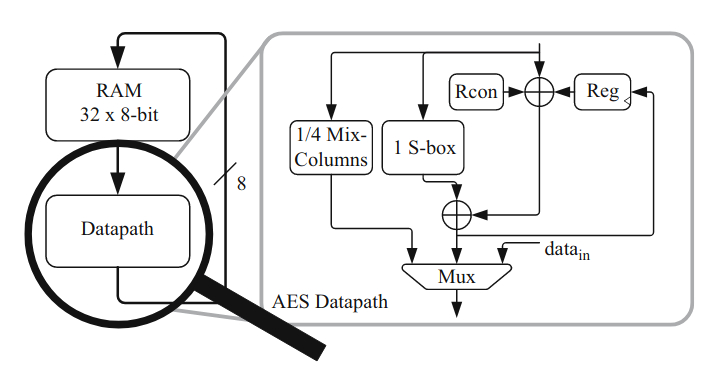
\includegraphics[width=0.5\textwidth]{img/AES.png}}
\caption{Architektur eines 8-Bit AES Moduls \cite{b9}}
\label{fig6}
\end{figure}

Der Datenpfad-Block in der Fig. \ref{fig6} ist für die grundlegenden Berechnungen zuständig, die für die Verschlüsselung und Entschlüsselung mittels AES Verfahren notwendig sind. Diese grundlegenden Berechnungen sind SubBytes, ShiftRows, MixColumns, AddRoundKey, InvSubBytes,  InvShiftRows und InvMixColumns. Diese Berechnungen arbeiten beim AES Verfahren mit einer Schlüssellänge von 128 Bit auf einer 4x4 Byte Matrix. Der 32x8 Bit = 128 Bit RAM enthält während der Laufzeit einen Zustand von 128 Bit als 4x4 Byte Matrix und einen 128 Bit Rundenschlüssel.

Neben AES gibt es weitere Verschlüsselungsverfahren, welche sich eigenen um auf einem RFID Transponder eingesetzt zu werden. Das AES Verschlüsselungsverfahren ist an der Stelle lediglich ein Beispiel für ein gängiges Verfahren. Jedoch ist nicht jedes Verfahren gleich sicher und es gibt jeweils zu jedem Verfahren vor und Nachteile. Diese müssen für jedes RFID System bei der Planung mit berücksichtigt werden. Durch den Einsatz guter Verschlüsselung wird das Mitlesen von Kommunikation zwischen Lesegerät und Transponder unterbunden. Durch dieses Unterbinden der Möglichkeit, die Kommunikation zwischen Lesegerät und Transponder mitzulesen, wird auch die Gefahr durch Man-In-The-Middle Angriffe verhindert. Dies liegt daran, dass ein sinnvoller Man-In-The-Middle Angriff darauf beruht die Kommunikation mitzulesen und bestimmte Stellen der Übertragung zu manipulieren. Durch Verschlüsselung kann ein Angreifer den Datenstrom ohne Kenntnis des Schlüssels nicht mehr sinnvoll manipulieren.

\section{Durchführbarkeit der Angriffe}
Nachdem nun zu den Schwachstellen passende Sicherheitsvorkehrungen vorgestellt wurden, wird an dieser Stelle diskutiert wie durchführbar die vorgestellten Angriffe sind und welche praktische Relevanz diese haben. Dazu wird in diesem Abschnitt für jeden der vorgestellten Angriffsszenarien aus Abschnitt IV separat diskutiert wie durchführbar und relevant diese Angriffe sind.

\subsection{Kopieren von Transpondern}
Das Kopieren von Transpondern ist grundsätzlich ein sehr leicht durchzuführender Angriff, welcher unbemerkt innerhalb weniger Sekunden durchgeführt werden kann, indem beispielsweise ein mittels eines kurzen Kontaktes mit einem liegengebliebenen Schlüsselbund oder Brieftasche die RFID Transponder kopiert werden können. Jedoch besitzen heutzutage die meisten Transponder, wie beispielsweise in Karten zum kontaktlosen Bezahlen oder Transpondern zum öffnen von Türschlössern, wirkungsvolle Authentifizierungsmaßnahmen um ein Kopieren oder nicht autorisiertes Auslesen zu verhindern. Benutzt jedoch ein wichtiges System noch Transponder ohne Authentifizierung stellt das ein erhebliches Sicherheitsrisiko dar.

\subsection{Kompromittieren des Lesegerätes}
Der Angriff mittels Schadcode auf den Transponder hat ein hohes Schadenspotential. Ist es nicht leicht eine beispielsweise SQL Injection mittels RFID Transponder durchzuführen. Zum einen sollten die Daten eines RFID Transponders wie Nutzerdaten behandelt werden, was bedeutet, dass diese nicht ohne Vorverarbeitung in tiefere Systembereiche wie Datenbanken vordringen können. Eine weitere Hürde ist, dass der RFID Transponder überhaupt erst von einem Lesegerät gelesen werden muss. Dies ist bei einem Lesegerät, welches eine Authentifikation mit dem Transponder durchführt, sehr schwer umzusetzen ohne die Identität eines gültigen Transponders zu stehlen. Damit ist es nur schwer durchführbar ein System mittels eines RFID Transponders zu kompromittieren.

\subsection{Erweitern von NFC zu Bluetooth}
Die Durchführbarkeit dieses Angriffes hängt stark von der Vorsicht der Nutzer ab, welche das Smartphone oder NFC fähige Gerät benutzen. Die Koppelung selbst ist durch die geringe Reichweite von NFC beim Koppeln verhältnismäßig sicher. Und es ist durch die Koppelung mittels NFC nicht mehr nötig ein Passwort für die Bluetooth-Verbindung einzugeben, welches potentiell ein Angriffspunkt für Brute-Force Angriffe war. Jedoch wenn ein Nutzer eines Smartphones unvorsichtig Bluetooth-Verbindungen mit unbekannten Geräten per NFC koppelt, können von diesen unbekannten Geräten durchaus ein Schadenspotential ausgehen.

\subsection{Tracking durch Transponder IDs}
Ein weitaus durchführbarer Angriff und Bedrohung für die Privatsphäre der Nutzer ist das Tracking mittes Transponder IDs. Dabei ist die Frage ob das Tracking durch einen Angriff von außerhalb erfolgen soll oder aber ein System bewusst so designt wird, dass es Tracking ermöglicht.

Prinzipiell ist es relativ leicht Tracking für außenstehende Angreifer zu untersagen, indem man, wie im Kapitel "Schutzmaßnahmen" skizziert, dafür sorgt, dass sich die übermittelte ID eines Transponders bei jedem Leseversuch ändert. Dabei ist es egal ob vollständig zufällige IDs generiert werden oder mittels randomisierten HashLock Verfahrens die IDs generiert werden. Wichtig ist nur, dass dabei für einen Außenstehenden bei jedem Auslesen eine andere ID übermittelt wird.

Soll jedoch innerhalb eines Systems das Tracking ermöglicht werden, bieten sich Verfahren wie das HashLock Verfahren an um die Transponder innerhalb eines Systems verfolgen zu können. Damit ist Gefahr durch Tracking aber bewusst in ein  System implementiert worden und dadurch ist das Tracking innerhalb dieses Systems sehr leicht durchführbar.


\subsection{Denial of Service Angriffe}
Ein ebenfalls leicht durchführbarer Angriff ist der Denial of Service Angriff bei dem der Transponder vor dem Lesegerät abgeschirmt wird. Diese Schwachstelle von RFID ist leicht durchzuführen, da es im Handel RFID blockierende Beutel zu kaufen gibt, welche im wesentlichen einen Faradayschen Käfig darstellen. In diesen Beuteln werden RFID Transponder nicht mit Energie versorgt, wenn sich ein Lesegerät in der Nähe befindet, da diese Beutel das elektrische Feld des Lesegerätes abschirmen. Neben der leichten Durchführbarkeit hat dieser Angriff auch ein hohes Schadenspotential wenn man das Szenario einer Diebstahlsicherung in Betracht zieht. Eine Diebstahlsicherung mittels RFID Transpondern kann damit sehr leicht umgangen werden und einen hohen Schaden bei dem Ladenbesitzer erzeugen.

\subsection{Abhören der Kommunikation / Man-In-The-Middle Angriff}
Die Schwachstelle dass sich RFID Kommunikation leicht abhören lässt, da die Kommunikation unverschlüsselt stattfindet, hat zu verschiedenen Problemen geführt. Zum einen ermöglicht es bei manchen Authentifizierungsprotokollen das mitlesen wichtiger Schlüssel oder Informationen. Zum anderen ermöglicht diese Schwachstelle aber auch die Durchführung von Man-In-The-Middle Angriffen. Um die Durchführbarkeit dieser Angriffe bewerten zu können müssen verschiedene Punkte betrachtet werden.

Zum einen wird je nach verwendeter RFID Technik eine gewisse Nähe zum Lesegerät und Transponder benötigt um die Kommunikation mitschneiden zu können. Besonders bei NFC mit der Reichweite von bis zu 10 cm ist das ein Problem. Dadurch ist es sehr schwer unbemerkt die Kommunikation abzuhören oder einen Man-In-The-Middle Angriff durchzuführen.

Zum anderen stellt die Verwendung von Verschlüsselung ein enormes Problem für diese Technik dar. Wenn eine Kommunikation zwischen Lesegerät und Transponder verschlüsselt ist muss der Angreifer sowohl beim einfachen Abhören, als auch beim Man-In-The-Middle Angriff die verwendeten Schlüssel kennen um einen sinnvollen Angriff durchzuführen.

Aus diesen beiden genannten Gründen ist es nicht besonders leicht einen unbemerkten und sinnvollen Abhörangriff oder einen Man-In-The-Middle Angriff mittels RFID Technik durchzuführen. Jedoch hängt dies stark von der verwendeten Technik ab. RFID Transponder mit einer hohen Reichweite und keiner Verschlüsselung würden die Durchführbarkeit der Angriffe erhöhen.

\section{Fazit}
Die kontaktlose RFID Technik bietet eine Vielzahl an Möglichkeiten wie beispielsweise der Komfort beim kontaktlosen Bezahlen oder die Möglichkeit Waren, nahezu unsichtbar, vor Diebstahl zu sichern. Jedoch müssen bei dem entwerfen eines RFID Systems die vorgestellten Schwachstellen in Betracht gezogen werden und für das zu entwickelnde System sinnvolle Sicherheitsmaßnahmen getroffen werden. Dies ist zwingend erforderlich, um die Angriffsfläche zu minimieren und die Durchführbarkeit von Angriffen zu erschweren. Des Weiteren sollte, je nach Anwendung, die Privatsphäre der Nutzer in Betracht gezogen werden und ebenfalls Schutzmaßnahmen ergriffen werden, um beispielsweise ein Tracking und ein Auslesen von sensiblen personenbezogenen Daten aus dem Transponder verhindern.

\begin{thebibliography}{00}
\bibitem{b1} Chih-Yung Chen, Chien-Ping Kuo and Fang-Yuan Chien, "An exploration of RFID information security and privacy," 2009 Joint Conferences on Pervasive Computing (JCPC), Tamsui, Taipei, 2009, pp. 65-70, doi: 10.1109/JCPC.2009.5420211.

\bibitem{b2} N. A. Chattha, "NFC — Vulnerabilities and defense," 2014 Conference on Information Assurance and Cyber Security (CIACS), Rawalpindi, 2014, pp. 35-38, doi: 10.1109/CIACS.2014.6861328.

\bibitem{b3} G. Madlmayr, J. Langer, C. Kantner and J. Scharinger, "NFC Devices: Security and Privacy," 2008 Third International Conference on Availability, Reliability and Security, Barcelona, 2008, pp. 642-647, doi: 10.1109/ARES.2008.105.

\bibitem{b4} NPX Semiconductors (32, November 2017) MIFARE Classic EV1 4K - Mainstream contactless smart card IC for fast and easy solution development. [Online]. Available: https://www.nxp.com/docs/en/data-sheet/MF1S70YYX\_V1.pdf.

\bibitem{b5} M. R. Rieback, B. Crispo and A. S. Tanenbaum, "Is your cat infected with a computer virus?," Fourth Annual IEEE International Conference on Pervasive Computing and Communications (PERCOM'06), Pisa, 2006, pp. 10 pp.-179, doi: 10.1109/PERCOM.2006.32.

\bibitem{b6} R. Verdult and F. Kooman, "Practical Attacks on NFC Enabled Cell Phones," 2011 Third International Workshop on Near Field Communication, Hagenberg, 2011, pp. 77-82, doi: 10.1109/NFC.2011.16.

\bibitem{b7} S. Skowron, Animation zur Ladungsverschiebung bei einem faradayschen Käfig. [Online]. Available: https://commons.wikimedia.org/ wiki/File:Faraday\_cage.gif\#/media/Datei:Faraday\_cage.gif

\bibitem{b8} G. Kulkarni, R. Shelke, R. Sutar and S. Mohite, "“RFID security issues \& challenges”," 2014 International Conference on Electronics and Communication Systems (ICECS), Coimbatore, 2014, pp. 1-4, doi: 10.1109/ECS.2014.6892730.

\bibitem{b9} P. Kitsos and Y. Zhang, "RFID Security: Techniques, Protocols and System-on-Chip Design", DOI: 10.1007/978-0-387-76481-8

\end{thebibliography}
\end{document}
